\documentclass{standalone}
\listfiles
\usepackage{tikz}
\usepackage{amsmath}
\usetikzlibrary{intersections,calc,angles} % 変更点:交点を求めるために追加

\begin{document}

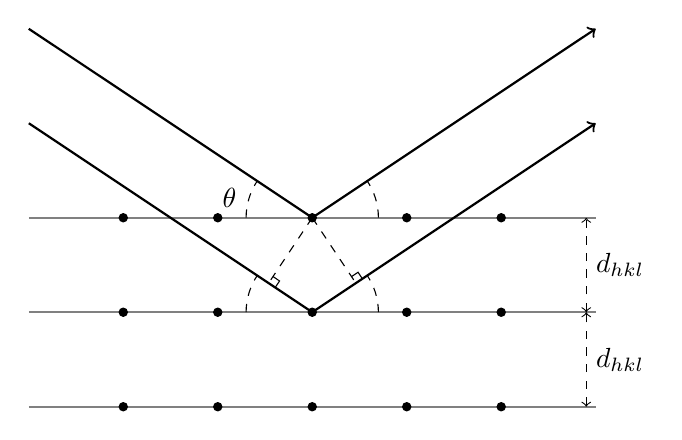
\begin{tikzpicture}[scale=1.2]
  % 結晶面
  \foreach \y in {0, 1, 2} {
    \draw[gray, thick] (-3,\y) -- (3,\y);
  }

  % 反射点(x=0)
  \coordinate (P1) at (0,1);
  \coordinate (P2) at (0,2);

  % 入射光と反射光(下)
  \draw[thick] (-3,3) -- (P1);
  \draw[thick,->] (P1) -- (3,3);

  % 入射光と反射光(上)
  \draw[thick] (-3,4) -- (P2);
  \draw[thick,->] (P2) -- (3,4);

  % 入射角と反射角(下)
  \draw[dashed] (P1) ++(0.7,0) arc[start angle=0 ,end angle=33.68,radius=0.7];
  \draw[dashed] (P1) ++(-0.7,0) arc[start angle=180, end angle=146.31, radius=0.7];

  % 入射角と反射角(上)
  \draw[dashed] (P2) ++(0.7,0) arc[start angle=0 ,end angle=33.68,radius=0.7];
  \draw[dashed] (P2) ++(-0.7,0) arc[start angle=180, end angle=146.31, radius=0.7];

  % theta ラベル(上の入射角)
  \node [anchor=south east] at (-0.7,2) {$\theta$};

  % dのマーク
  \draw[<->,dashed] (2.9,0) -- (2.9,1);
  \draw[<->,dashed] (2.9,1) -- (2.9,2);
  \node[right] at (2.9,0.5) {$d_{hkl}$};
  \node[right] at (2.9,1.5) {$d_{hkl}$};

  % 原子の点
  \foreach \x in {-2,-1,0,1,2} {
    \foreach \y in {0,1,2} {
      \fill[black] (\x,\y) circle (0.05);
    }
  }
  \coordinate (R1) at (3,3);
  \coordinate (Q1) at ($(P1)!(P2)!(R1)$);
  \path let \p1 = (Q1) in coordinate (Q2) at ({-\x1}, \y1);
  \draw[dashed] (P2) -- (Q1);
  \draw[dashed] (P2) -- (Q2);
  \coordinate (R1) at (3,3);
  \draw pic [draw,angle radius=0.1cm] {right angle=P2--Q1--R1};
  \draw pic [draw,angle radius=0.1cm] {right angle=P2--Q2--P1};


\end{tikzpicture}


\end{document}
